% !TeX program = lualatex

\documentclass[12pt]{article}



\usepackage[margin=1in]{geometry} 
\usepackage{amsmath,amsthm,amssymb}
\usepackage{MnSymbol}
\usepackage{graphicx}
\usepackage{bm}
\usepackage[normalem,normalbf]{ulem}
\usepackage{algorithm} 
\usepackage{algpseudocode} 
\usepackage{multirow}
\usepackage{rotating}
\usepackage{therefore}

\usepackage{tikz}
\usetikzlibrary{shapes.multipart}
\usetikzlibrary{shapes.symbols}

\usetikzlibrary{graphs,graphdrawing,graphs.standard,quotes}
\usegdlibrary{circular,force,layered,routing}
\tikzset{
	graphs/simpleer/.style={
		nodes={draw,circle, blue, left color=blue!20, text=black, inner sep=1pt},
		node distance=2.5cm, nodes={minimum size=2em}
	},
	every loop/.style={},
}

\newcommand*\circled[1]{\tikz[baseline=(char.base)]{
		\node[shape=circle,draw,inner sep=2pt] (char) {#1};}}

\newcommand{\m}{\medskip\\}
\newcommand{\N}{\mathbb{N}}
\newcommand{\Z}{\mathbb{Z}}
\newcommand{\R}{\mathbb{R}}
\newcommand{\bbs}{\textbackslash\textbackslash\space}
\newcommand{\bs}{\textbackslash\space}
\newcommand{\la}{\enskip\land\enskip}
\newcommand{\lo}{\enskip\lor\enskip}
\newcommand{\comp}[1]{#1^\mathsf{c}}
\newcommand{\micdrop}{\qed}
\newcommand{\contra}{\begin{tikzpicture}
		\node[starburst, draw, minimum width=3cm, minimum height=2cm,line width=1.5pt,red,fill=yellow,scale=.5]
		{BOOM, A CONTRADICTION!!!};
\end{tikzpicture}}

\renewcommand{\qedsymbol}{$\blacksquare$}

\DeclareMathOperator{\lcm}{lcm}

\newtheorem{theorem}{Theorem}

\newenvironment{exercise}[2][Exercise]{\begin{trivlist}
		\item[\hskip \labelsep {\bfseries #1}\hskip \labelsep {\bfseries #2.}]}{\end{trivlist}}

\setlength\parindent{24pt}

\makeatletter
\renewcommand*\env@matrix[1][*\c@MaxMatrixCols c]{%
	\hskip -\arraycolsep
	\let\@ifnextchar\new@ifnextchar
	\array{#1}}
\makeatother



\begin{document}
	
	% --------------------------------------------------------------
	%                         Start here
	% --------------------------------------------------------------
	
	
	\title{Homework 2 (Due Jan 25, 2023)}
	\author{Jack Hyatt\\ %replace with your name
		MATH 575 - Discrete Mathamatics II - Spring 2023} 
	
	\maketitle
	
	Justify all of your answers completely.\\
	
	
	\medskip 
	
	
	
	\begin{enumerate}

\item Recall that $\Delta(G)$ and $\delta(G)$ denote the maximum degree and minimum degree of a graph $G$ respectively. Suppose $G$ has $n$ vertices.
\begin{enumerate}
\item Prove that if $\delta(G) \geq \lceil (n-1)/2 \rceil$, then $G$ is connected.
\begin{proof}
	Assume $\delta(G) \geq \lceil (n-1)/2 \rceil$. Assume towards contradiction that G has at least 2 connected components. WLOG, let A be the connected component with the least number of vertices. So $|V(A)|\leq \lfloor\frac{n}{2}\rfloor$. Let $v_a$ be the vertex s.t. $\delta(A) = d(v_a)$. We have $d(v_a)\geq \delta(G)$, so $d(v_a)\geq \lceil (n-1)/2 \rceil$ and $d(v_a)\leq \lfloor\frac{n}{2}\rfloor-1$
	\[\lceil (n-1)/2 \rceil \leq d(v_a)\leq \lfloor\frac{n}{2}\rfloor-1\]
	\[\bigg\lceil \frac{n}{2}-\frac{1}{2} \bigg\rceil \leq \bigg\lfloor \frac{n}{2}-1 \bigg\rfloor\]
	This is false for all values of $n$.\contra\\
	So G cannot have at least 2 connected components.
\end{proof}
\item For all $n \geq 3$, give an example of an $n$-vertex disconnected graph  $G$ with $\delta(G) = \lfloor (n-2)/2 \rfloor$.
\begin{proof}
	Assume G is a graph and has $n\geq3$ vertices.\\
	Case 1: $n$ is even.\\
	Since $n$ is even, $2k = n$ for some $2\leq k\in\N$. Let G have two connected components, $A$ and $B$, with both having $k$ vertices. Let's make both of them complete subgraphs. Then the lowest degree of a vertex will be $k-1 = (2k-2)/2 = \lfloor (n-2)/2 \rfloor$.\\\\
	Case 2: $n$ is odd.\\
	Since $n$ is odd, $2k+1 = n$ for some $1\leq k\in\N$. Let G have two connected components, $A$ and $B$, with $k$ and $k+1$ vertices respectively. Let's make both of them complete subgraphs. Then the lowest degree of a vertex will be in $A$, namely $k-1 = \lfloor k-1 \rfloor =\lfloor (2k+1-3)/2 \rfloor = \lfloor (n-2)/2 - (1/2)\rfloor = \lfloor (n-2)/2 \rfloor$, since $n$ is odd.\\\\
\end{proof}
\item Prove or disprove: if $\delta(G) = \lfloor (n-2)/2 \rfloor$ and $\Delta(G) \geq \lceil n/2 \rceil$, then $G$ is connected.  
\begin{proof}
	Assume G is a graph, $\delta(G) = \lfloor (n-2)/2 \rfloor$ and $\Delta(G) \geq \lceil n/2 \rceil$. Assume towards contradiction that G has at least two connected components.\\
	\textbf{Case 1}: $n$ is even.\\
	Since $n$ is even, $n=2k$ for some $k\in\N$, and $\delta(G) = k-1$ and $\Delta(G) \geq k$. WLOG, let us consider two connected components of $G$, called $A$ and $B$, and let $A$ contain a vertex with the maximum degree. So $A$ must contain at least $k+1$ vertices. So then $B$ can at most contain $k-1$ vertices. So in $B$, the max degree a vertex can have is $k-2$, but this is less than $\delta(G)$.\contra\\\\
	\textbf{Case 2}: $n$ is odd.\\
	Since $n$ is odd, $n=2k+1$ for some $k\in\N$, and $\delta(G) = \lfloor (2k-1)/2 \rfloor=\lfloor k-(1/2) \rfloor = k-1$ and $\Delta(G) \geq \lceil (2k+1)/2 \rceil = \lceil k+(1/2) \rceil =k+1$. WLOG, let us consider two connected components of $G$, called $A$ and $B$, and let $A$ contain a vertex with the maximum degree. So $A$ must contain at least $k+2$ vertices. This means $B$ contains $k-1$ vertices. So the highest degree a vertex in $B$ can have is $k-2$, but this is less than $\delta(G)$. \contra
	
\end{proof}
\end{enumerate}
\medskip


\item Prove that if $G$ is an $n$-vertex bipartite graph, then $|E(G)| \leq \frac{n^2}{4}$.
\begin{proof}
	Let $G$ be a bipartite graph, partitioned into $X$ and $Y$, with $n$ total vertices. So then $|X|+|Y|=n$, and $|E(G)| \leq |X|\cdot|Y|$. One upper bound for $|E(G)|$ is the maximum for $|X|\cdot|Y|$. Maximizing $|X|\cdot|Y|$ with the condition $|X|+|Y|=n$ is a standard optimization problem taught in any Calculus course. Solving this optimization problem, we get the result $|X|=|Y|=\frac{n}{2}$, with $|X|\cdot|Y| = \frac{n^2}{4}$ as the maximum. 
\end{proof}
\medskip

\item A graph is called $k$-partite if its vertex set can be partitioned into sets $V_1, V_2, \ldots, V_k$ such that for each $1\leq i \leq k$, there are no edges between vertices in the set $V_i$. Prove that for all integers $k \geq 2$ every graph  $G$ has a $k$-partite subgraph with at least $\frac{(k-1)|E(G)|}{k}$ edges.



\begin{proof}
	Let us induct on $n$, the number of vertices.\\
	\textbf{Base case}: $n=1$\\
	This is so obvious, that one wouldn't even need a PhD to see.\\
	\textbf{Induction Step}: Assume G is a graph with $n$ vertices. Assume the claim in the problem holds for any graph with $n'$ vertices where $1\leq n'<n$.\\
	Choose the vertex that just got out of solitary confinement, $v$, and throw them back in there (remove it from the graph), and now we have a subgraph $H$, with $n-1$ vertices. $|V(H)| < n$, so we know that the induction hypothesis holds for $H$. So there is a subgraph, $H'$, with $k$ partitions with at least
	$|E(H)|-\frac{|E(H)|}{k}$ edges. Now, let us release $v$ from solitary confinement back into society, with the same social connections it had before, except for a key difference. Let us place $v$ into the partiotion $V_i$, s.t. the number of edges between $v$ and the vertices in $V_i$ is the least out of all $V_1,V_2,\ldots,V_k$ (if there are multiple as the minimum, any work). Let $m$ be the number of edges incident to $v$ and that minimum $V_i$. Note: $m\leq \frac{d(v)}{k}$\\
	$v$ will keep the edges it has with the other partitions, but we will remove the edges it shared with vertices in the partition we placed it in. Let us call this subgraph of $G$, $G'$.
	\begin{align*}
		|E(G')| &= |E(H')|+d(v)-m\\
		&\geq |E(H')|+d(v)-\frac{d(v)}{k} &&&\text{From the 'Note'}\\
		&=|E(H')| + \frac{(k-1)|d(v)}{k}\\
		&\geq\frac{(k-1)|E(H)|}{k} + \frac{(k-1)|d(v)}{k} &&& \text{From Induction Hypothesis}\\
		&=\frac{k-1}{k}\cdot(|E(H)|+d(v))\\
		&=\frac{k-1}{k}\cdot |E(G)|\\\\
		\therefore |E(G')| &\geq \frac{k-1}{k}\cdot |E(G)|
	\end{align*} 
\end{proof}


\medskip

\item Consider the graph $G$ below.
\begin{center}
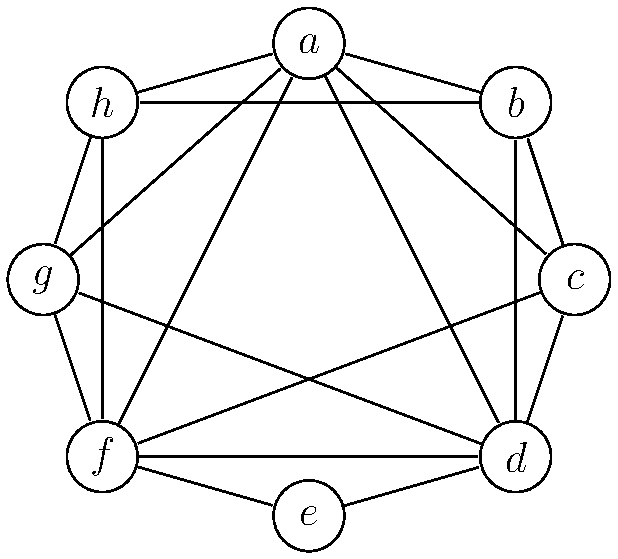
\includegraphics[scale=.5]{4_2.pdf}
\end{center}

\begin{enumerate}
\item Partition the edge set of $G$ into a collection of edge-disjoint cycles. List the vertices of each cycle.\\\\
(a,b,c,d,e,f,g,h,a)\\
(b,d,f,h,b)\\
(a,d,g,a)\\
(a,c,f,a)\\

\item Splice together the cycles in part (a) to find an Eulerian circuit of $G$.\\\\
Start with first cycle: (a,b,c,d,e,f,g,h,a)\\
Splice in second: (a,b,d,f,h,b,c,d,e,f,g,h,a)\\
Add in third at end: (a,b,d,f,h,b,c,d,e,f,g,h,a,d,g,a)\\
Add in fourth at end: (a,b,d,f,h,b,c,d,e,f,g,h,a,d,g,a,c,f,a)\\
\end{enumerate}



\medskip

\item Determine if each of the following sequences is graphic. If it is not, give a reason why. If it is, draw a graph that realizes the degree sequence.\\\\
I will use Havel-Hakimi theorem.
\begin{enumerate}
\item $(4,4,3,3,2,2,1,1,1)$\\
Not graphic since there is an odd number of odd numbers.
\item $(4,4,3,3,2,2,1,1)$\\
$(3,2,2,2,1,1,1)$\\
$(1,1,1,1,1,1)$\\
This is graphic, so the other is graphic.\\

\begin{center}
	\begin{tikzpicture}[scale=.75]
		\graph[simpleer, simple necklace layout]{
			1--{2};
			2--{1};
			3--{4};
			4--{3};
			5--{6};
			6--{5};
			7--{1,2,3};
			8--{7,1,2,3};
		};
	\end{tikzpicture}
\end{center}

\item $(8,7,6,5,4,3,2,1)$\\
Not graphic since there is a vertex with degree 8 and only 7 other vertices to be neighbors.
\item $(7,4,4,4,4,3,3,3)$\\
$(3,3,3,3,2,2,2)$\\
$(2,2,2,2,2,2)$\\
$(2,2,2,1,1)$\\
$(1,1,1,1)$\\
This is graphic, so the other is graphic.\\
\begin{center}
	\begin{tikzpicture}[scale=.75]
		\graph[simpleer, simple necklace layout]{
			1--{2};
			2--{1};
			3--{4};
			4--{3};
			5--{1,2};
			6--{3,4};
			7--{1,2,3};
			8--{1,2,3,4,5,6,7};
		};
	\end{tikzpicture}
\end{center}

\end{enumerate}

\end{enumerate}
\end{document}
